\documentclass[final,hyperref={pdfpagelabels=false}]{beamer}
\usepackage{grffile}
\mode<presentation>{\usetheme{PosterLogProb}}
\usepackage[english]{babel}
\usepackage[utf8]{inputenc}
\usepackage{amsmath,amsthm, amssymb, latexsym}
\usepackage{epsfig}
\usepackage{listings}
\usepackage{lstlinebgrd}

\usepackage[orientation=portrait,size=a0,scale=1.4,debug]{beamerposter}
\providecommand\thispdfpagelabel[1]{}
\setbeamertemplate{bibliography entry title}{\color{black}}
\setbeamertemplate{bibliography entry location}{}
\setbeamertemplate{bibliography entry note}{}

\usepackage{array,booktabs,tabularx}
\newcolumntype{Z}{>{\centering\arraybackslash}X} % centered tabularx columns
\newcommand{\pphantom}{\textcolor{ta3aluminium}} % phantom introduces a vertical space in p formatted table columns??!!

\listfiles

\usepackage{amsthm}
%%%%%%%%%%%%%%%%%%%%%%%%%%%%%%%%%%%%%%%%%%%%%%%%%%%%%%%%%%%%%%%%%%%%%%%%%%%%%%%%%%%%%%


 \title{\huge\bfseries\hspace*{-1em} Empurrando Juntos\\(Pushing Together)\\A platform for social participation}
\date{}
\author{\large Tallys Martins
\and Dylan Guedes
\and Luan Guimarães \\
\and Ricardo Poppi
\and Henrique Parra
\and Paulo Meirelles
}
\institute[UNB/CD]{University of Brasília and Cidade Democrática Institute, Brazil}

\newlength{\columnheight}
\setlength{\columnheight}{105cm}


\begin{document}
\setbeamertemplate{caption}{\raggedright\insertcaption\par}
\begin{frame}
  \begin{columns}
    % ---------------------------------------------------------%
    % Set up a column
    \begin{column}{.49\textwidth}
      \begin{beamercolorbox}[center,wd=\textwidth]{postercolumn}
        \begin{minipage}[T]{.95\textwidth}
          \parbox[t][\columnheight]{\textwidth}{

\begin{block}{Bubbles of Opinion}
  \begin{itemize}

    \item Civic tech platforms with threaded architecture are a barrier for
    engagement of regular and lay people

    \item Popular social media recommendation algorithms are black boxes 
    oriented by business interests

    \item Engines and systems are specialized in analyzing our profiles. We only receive
    content about what we like, what we follow and what our friends see

    \item People are stuck in a phenomenon that we call ``bubbles of opinion'' where
    their opinions do not reach people outside their group

    \item The bubbles caused by this algorithms unbalance the dialog and minorities
    are despised in reacting to misinformation and fake news
  \end{itemize}
\end{block}

\begin{block}{Polis}
  \begin{itemize}
    \item Polis is a web based platform for online debates that uses A.I. to
    show the different opinion groups in a discussion

    \item Allows people to create online conversations to debate about any subject,
    anonymous or not, and uses a different approach to build the dialog between users

    \item Using a concept that we call ``crowdsource participation'', people can
    give their opinions by simply clicking in ``agree'', ``disagree'' or ``skip''
    in other  comments. Participation gets easier in a one click effort, with
    potential of engaging thousands

    \item The system applies clustering algorithms to identify the different groups
    of opinion based on the reactions of the participants in the comments

    \item The majority and minority consensus is shown in a graph, and can be
    displayed either in the global scope considering all the participants or in each group
    scope
  \end{itemize}

  \begin{figure}
    \begin{center}
      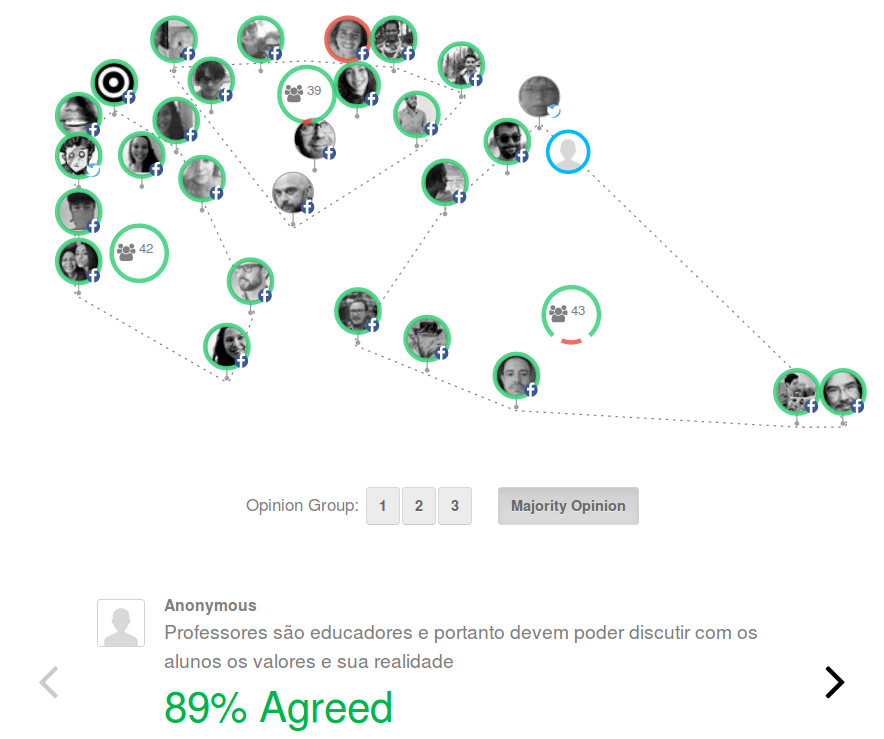
\includegraphics[scale=1.1]{../images/polis3.png}
      \caption{Groups of opinion formed by Polis about Brazilian education reform.}
      \label{fig:group-clusters}
    \end{center}
  \end{figure}
\end{block}

\begin{block}{What is Empurrando Juntos (EJ)?}

  \begin{itemize}
    \item A Free Open Source Software for social participation that aims to
    increase communication between majority and minority, blowing ``bubbles of
    opinion''

    \item A platform built on top of Polis that offers new features
    by using gamification concepts

    \item A tool that allows activists and non-extremist people to engage regular
    people in online discussions
  \end{itemize}
\end{block}

\begin{block}{Why EJ?}
  \begin{itemize}
    \item EJ goes beyond Polis by adding new features that offer more interaction
    to the discussions

    \item Uses gamification to explore the different profiles of participants
    as a mean to bring diversity to online discussions
  \end{itemize}
\end{block}


%-------------------------------------------------------------------------------
}
\end{minipage}
\end{beamercolorbox}
\end{column}
% ---------------------------------------------------------%
% end the column

% ---------------------------------------------------------%
% Set up a column
\begin{column}{.49\textwidth}
  \begin{beamercolorbox}[center,wd=\textwidth]{postercolumn}
    \begin{minipage}[T]{.95\textwidth} % tweaks the width, makes a new \textwidth
      \parbox[t][\columnheight]{\textwidth}{ % must be some better way to set the the height, width and textwidth simultaneously

\begin{block}{EJ Features}
  \begin{itemize}
    \item Uses Polis engine to obtain the groups of opinion

    \item Provides a resource that we called ``the Push''. People in ownership of
    this ability (gamification) can access special features in the platform

    \item ``The Push'' is given to special actors in the groups formed by Polis.
    Three profiles are considered: the activist, the bridge, and the consultation
    owner participants and give them

    \item Monitors Polis conversations created through an App
    to identify activists and bridge participants, giving them ``the Push''
    power
  \end{itemize}

\end{block}

\begin{block}{Profiles identified by EJ}
  \begin{figure}
    \begin{center}
      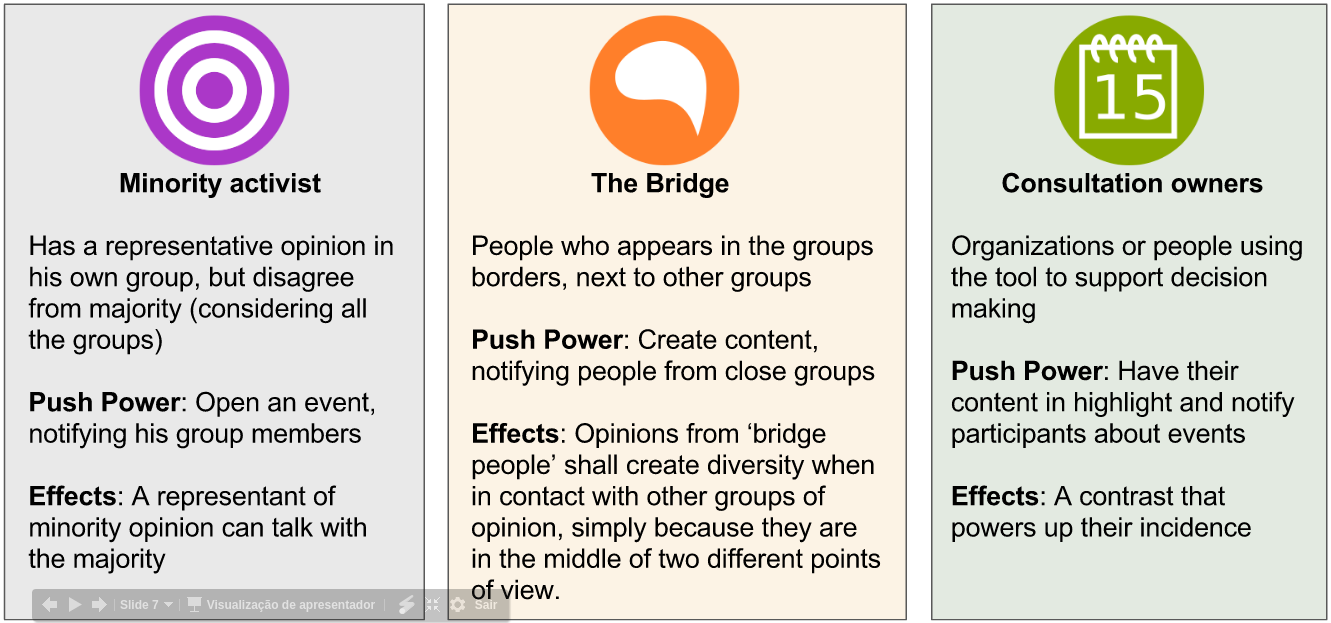
\includegraphics[scale=1.45]{../images/userprofiles.png}
      \caption{}
      \label{fig:user-profiles}
    \end{center}
  \end{figure}
\end{block}

\begin{block}{EJ System Architecture}

  \begin{figure}
    \begin{center}
      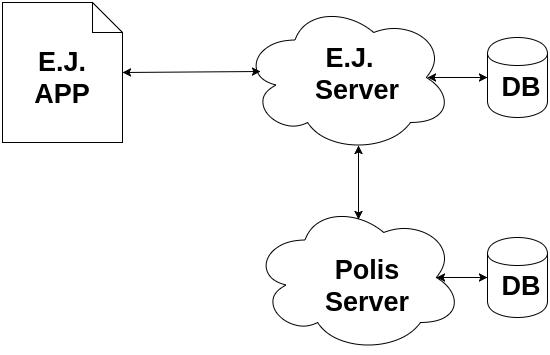
\includegraphics[scale=1.3]{../images/polis4.png}
      \label{fig:architecture}
    \end{center}
  \end{figure}

	\begin{itemize}
    \item Front-end application, written in React Native
    and a NodeJS server.

    \item The server module is responsible for managing users, ``the Push'', and
    to make the interface with Polis API.
  \end{itemize}

\end{block}

\begin{block}{Integration with Polis}
  \begin{itemize}
    \item Other platforms can register the participation of their users on Polis
    through the xID (external id) parameter in the API

    \item Polis conversations can be easily embed with Javascript snippets

    \item EJ calculates the profiles based on the conversation data, and in the future this
    will be included in the core of the clusters math to provide it through an API
  \end{itemize}
\end{block}
\begin{block}{Final Remarks}
  \begin{itemize}
    \item EJ arises as a potential tool to bridge dialog between society and
    the state, making different analyses about the opinion of the distinct groups
    and also opening new possibilities for the expression of these opinions with ``the
    Push'' resource

    \item We are now working on a research to evolve the clustering service that
    will fit our application model. Our next steps include evolving the
    mobile application using mocked data and validating the user interface

    \item All our contributions are published in open repositories available at:
      \begin{itemize}
        \color{blue}
        \item \url{github.com/cidadedemocratica/pushingtogether}
        \item \url{github.com/cidadedemocratica/app_pushingtogether}
      \end{itemize}
  \end{itemize}
\end{block}
      }
        \end{minipage}
      \end{beamercolorbox}
    \end{column}
  \end{columns}
\end{frame}
\end{document}
